%kelompok 1 Sistem Operasi (firmata, komunikasi arduino)
%Kelas D4 TI 1B
%Adam Noer Hidayatullah 1174097
%Ichsan Hizman Hardy 1174034
%Teddy
%Nisrina Aulia
%Irvan Rizkiansyah 1174043

\section{Firmata, komunikasi arduino}

	\subsection{Firmata}
	Firmata adalah protocol yang ditulis pada Arduino untuk memudahkan komunikasi serial Arduino dengan sesama software di komputer. Firmata pun support berbagai macam sistem operasi tidak hanya pada windows saja, melainkan seperti linux, MacOSX pun support firmata. Dibawah ini adalah contoh test Firmata pada MacOSX.
	
	\begin{figure} [ht]
		\centerline{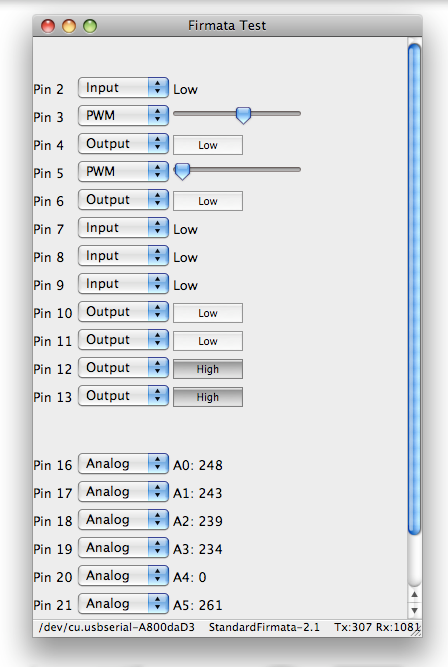
\includegraphics[width=1\textwidth]{figures/firmatates.png}}
		\caption{Gambar Contoh Test Firmata MacOSX}
		\label{firmatates}
	\end{figure}
	
	\ref{firmatates}
	
	
	\subsection{LabVIEW}
	LabVIEW memiliki fungsi yang sama seperti firmata tetapi lebih mudah, mudah dalam arti pemrograman tidak lagi dilakukan di kedua sisi,
	tetapi hanya di satu sisi, yaitu di software komputer saja.
	
	\subsection{Fungsi Firmata}
	contoh fungsi firmata adalah dapat mengontrol Arduino menggunakan software seperti LabVIEW, MATLAB, dll, tanpa harus memprogram khusus di Arduino.
	
	\subsection{MATLAB}
	MATLAB adalah salah satu software yang sepenuhnya mengambil kontrol pda arduino fungsinya akan menghemat waktu dalam mengintegrasi MATLAB arduino.
	
	\subsection{Interaksi Arduino dan LabVIEW}
	Interaksi Arduino dan LabVIEW yaitu kerena masing masing memiliki kelebihan dan kekurangan, apabila digabungkan keduanya akan saling menambahkan,
	sebaliknya kekurangan kekurangannya keduanya akan saling meniadakan.
	
	\subsection{Menginstall Firmata}
	Menginstal Firmata di LabVIEW disebut dengan LabVIEW Interface For Arduino (LVIFA). fungsingnya yaitu dapat membaca sinyal analog potensio,
	pembaca sensor seperti thermistor,LDR, joystick.